% !TeX spellcheck = pl_PL
%%%%%%%%%%%%%%%%%%%%%%%%%%%%%%%%%%%%%%%%%%%
%                                        %
% Szablon pracy dyplomowej inzynierskiej % 
% zgodny  z aktualnymi  przepisami  SZJK %
%                                        %
%%%%%%%%%%%%%%%%%%%%%%%%%%%%%%%%%%%%%%%%%%
%                                        %
%  (c) Krzysztof Simiński, 2018-2022     %
%                                        %
%%%%%%%%%%%%%%%%%%%%%%%%%%%%%%%%%%%%%%%%%%
%                                        %
% Najnowsza wersja szablonów jest        %
% podstępna pod adresem                  %
% github.com/ksiminski/polsl-aei-theses  %
%                                        %
%%%%%%%%%%%%%%%%%%%%%%%%%%%%%%%%%%%%%%%%%%
%
%
% Projekt LaTeXowy zapewnia odpowiednie formatowanie pracy,
% zgodnie z wymaganiami Systemu zapewniania jakości kształcenia.
% Proszę nie zmieniać ustawień formatowania (np. fontu,
% marginesów, wytłuszczeń, kursywy itd. ).
%
% Projekt można kompilować na kilka sposobów.
%
% 1. kompilacja pdfLaTeX
%
% pdflatex main
% bibtex   main
% pdflatex main
% pdflatex main 
%
%
% 2. kompilacja XeLaTeX
%
% Kompilatacja przy użyciu XeLaTeXa różni się tym, że na stronie
% tytułowej używany jest font Calibri. Wymaga to jego uprzedniego
% zainstalowania. 
%
% xelatex main
% bibtex  main
% xelatex main
% xelatex main 
%
%
%%%%%%%%%%%%%%%%%%%%%%%%%%%%%%%%%%%%%%%%%%%%%%%%%%%%%
% W przypadku pytań, uwag, proszę pisać na adres:   %
%      krzysztof.siminski(małpa)polsl.pl            %
%%%%%%%%%%%%%%%%%%%%%%%%%%%%%%%%%%%%%%%%%%%%%%%%%%%%%
%
% Chcemy ulepszać szablony LaTeXowe prac dyplomowych. 
% Wypełniając ankietę spod poniższego adresu pomogą 
% Państwo nam to zrobić. Ankieta jest całkowicie 
% anonimowa. Dziękujemy! 
% https://docs.google.com/forms/d/e/1FAIpQLScyllVxNKzKFHfILDfdbwC-jvT8YL0RSTFs-s27UGw9CKn-fQ/viewform?usp=sf_link
%
%%%%%%%%%%%%%%%%%%%%%%%%%%%%%%%%%%%%%%%%%%%%%%%%%%%%%%%%%%%%%%%%%%%%%%%%%

%%%%%%%%%%%%%%%%%%%%%%%%%%%%%%%%%%%%%%%%%%%%%%%
%                                             %
% PERSONALIZACJA PRACY – DANE PRACY           %
%                                             %
%%%%%%%%%%%%%%%%%%%%%%%%%%%%%%%%%%%%%%%%%%%%%%%

% Proszę wpisać swoje dane w poniższych definicjach.

% TODO
\newcommand{\FirstName}{Aleksander}
\newcommand{\Surname}{Mickiewicz}
\newcommand{\Supervisor}{Dr inż Michał Staniszewski}
\newcommand{\Title}{Renderowanie terenu metodą ray marching}
\newcommand{\TitleAlt}{Rendering terrain using ray marching method}
\newcommand{\Program}{Informatyka}            % kierunek studiów  (bez $\langle$ i $\rangle$)
\newcommand{\Specialisation}{Grafika komputerowa}
\newcommand{\Id}{293830}
\newcommand{\Departament}{}

% Jeżeli został wyznaczony promotor pomocniczy lub opiekun, proszę go/ją wpisać ...
\newcommand{\Consultant}{} % dane promotora pomocniczego, opiekuna (bez $\langle$ i $\rangle$)
% ... w przeciwnym razie proszę zostawić puste miejsce jak poniżej:
%\newcommand{\Consultant}{} % brak promotowa pomocniczego / opiekuna

% koniec fragmentu do modyfikacji
%%%%%%%%%%%%%%%%%%%%%%%%%%%%%%%%%%%%%%%%%%


%%%%%%%%%%%%%%%%%%%%%%%%%%%%%%%%%%%%%%%%%%%%%%%
%                                             %
% KONIEC PERSONALIZACJI PRACY                 %
%                                             %
%%%%%%%%%%%%%%%%%%%%%%%%%%%%%%%%%%%%%%%%%%%%%%%

%%%%%%%%%%%%%%%%%%%%%%%%%%%%%%%%%%%%%%%%  


%%%%%%%%%%%%%%%%%%%%%%%%%%%%%%%%%%%%%%%%%%%%%%%
%                                             %
% PROSZĘ NIE MODYFIKOWAĆ PONIŻSZYCH USTAWIEŃ! %
%                                             %
%%%%%%%%%%%%%%%%%%%%%%%%%%%%%%%%%%%%%%%%%%%%%%%



\documentclass[a4paper,twoside,12pt]{book}
\usepackage[utf8]{inputenc}                                      
\usepackage[T1]{fontenc}  
\usepackage{amsmath,amsfonts,amssymb,amsthm}
\usepackage[british,polish]{babel} 
\usepackage{indentfirst}



\usepackage{ifxetex}

\ifxetex
	\usepackage{fontspec}
	\defaultfontfeatures{Mapping=tex—text} % to support TeX conventions like ``——-''
	\usepackage{xunicode} % Unicode support for LaTeX character names (accents, European chars, etc)
	\usepackage{xltxtra} % Extra customizations for XeLaTeX
\else
	\usepackage{lmodern}
\fi



\usepackage[margin=2.5cm]{geometry}
\usepackage{graphicx} 
\usepackage{hyperref}
\usepackage{booktabs}
\usepackage{tikz}
\usepackage{pgfplots}
\usepackage{mathtools}
\usepackage{geometry}
\usepackage{subcaption}   % subfigures
\usepackage[page]{appendix} % toc,
\renewcommand{\appendixtocname}{Dodatki}
\renewcommand{\appendixpagename}{Dodatki}
\renewcommand{\appendixname}{Dodatek}

\usepackage{csquotes}
\usepackage[natbib=true,backend=bibtex]{biblatex}  % kompilacja bibliografii BibTeXem
%\usepackage[natbib=true,backend=biber]{biblatex}  % kompilacja bibliografii Biberem
\bibliography{biblio/biblio}

\usepackage{ifmtarg}   % empty commands  

\usepackage{setspace}
\onehalfspacing


\frenchspacing



%%%% TODO LIST GENERATOR %%%%%%%%%

\usepackage{color}
\definecolor{brickred}      {cmyk}{0   , 0.89, 0.94, 0.28}

\makeatletter \newcommand \kslistofremarks{\section*{Uwagi} \@starttoc{rks}}
  \newcommand\l@uwagas[2]
    {\par\noindent \textbf{#2:} %\parbox{10cm}
{#1}\par} \makeatother


\newcommand{\ksremark}[1]{%
{%\marginpar{\textdbend}
{\color{brickred}{[#1]}}}%
\addcontentsline{rks}{uwagas}{\protect{#1}}%
}

\newcommand{\comma}{\ksremark{przecinek}}
\newcommand{\nocomma}{\ksremark{bez przecinka}}
\newcommand{\styl}{\ksremark{styl}}
\newcommand{\ortografia}{\ksremark{ortografia}}
\newcommand{\fleksja}{\ksremark{fleksja}}
\newcommand{\pauza}{\ksremark{pauza `--', nie dywiz `-'}}
\newcommand{\kolokwializm}{\ksremark{kolokwializm}}
\newcommand{\cudzyslowy}{\ksremark{,,polskie cudzysłowy''}}

%%%%%%%%%%%%%% END OF TODO LIST GENERATOR %%%%%%%%%%%

%%%%%%%%%%%% ZYWA PAGINA %%%%%%%%%%%%%%%
% brak kapitalizacji zywej paginy
\usepackage{fancyhdr}
\pagestyle{fancy}
\fancyhf{}
\fancyhead[LO]{\nouppercase{\it\rightmark}}
\fancyhead[RE]{\nouppercase{\it\leftmark}}
\fancyhead[LE,RO]{\it\thepage}


\fancypagestyle{tylkoNumeryStron}{%
   \fancyhf{} 
   \fancyhead[LE,RO]{\it\thepage}
}

\fancypagestyle{bezNumeracji}{%
   \fancyhf{} 
   \fancyhead[LE,RO]{}
}

\fancypagestyle{NumeryStronNazwyRozdzialow}{%
   \fancyhf{} 
   \fancyhead[LE]{\nouppercase{\FirstName\ \Surname}}
   \fancyhead[RO]{\nouppercase{\leftmark}} 
   \fancyfoot[CE, CO]{\thepage}
}


%%%%%%%%%%%%% OBCE WTRETY  
\newcommand{\obcy}[1]{\emph{#1}}
\newcommand{\ang}[1]{{\selectlanguage{british}\obcy{#1}}}
%%%%%%%%%%%%%%%%%%%%%%%%%%%%%

% polskie oznaczenia funkcji matematycznych
\renewcommand{\tan}{\operatorname {tg}}
\renewcommand{\log}{\operatorname {lg}}

% jeszcze jakies drobiazgi

\newcounter{stronyPozaNumeracja}

%%%%%%%%%%%%%%%%%%%%%%%%%%% 
\usepackage{xstring}
\usepackage{ifthen}
\newcommand{\printOpiekun}[1]{%		

    \StrLen{\Consultant}[\mystringlen]
    \ifthenelse{\mystringlen > 0}%
    {%
       {\large{\bfseries OPIEKUN, PROMOTOR POMOCNICZY}\par}
       
       {\large{\bfseries \Consultant}\par}
    }%
    {}
} 
%
%%%%%%%%%%%%%%%%%%%%%%%%%%%%%%%%%%%%%%%%%%%%%%
 
% Proszę nie modyfikować poniższych definicji!
\author{\FirstName\ \Surname}
\newcommand{\Author}{\FirstName\ \MakeUppercase{\Surname}}
\newcommand{\Type}{PROJEKT INŻYNIERSKI}
\newcommand{\Faculty}{Wydział Automatyki, Elektroniki i Informatyki} 
\newcommand{\Polsl}{Politechnika Śląska}
\newcommand{\Logo}{graf/politechnika_sl_logo_bw_pion_pl.pdf}
\newcommand{\LeftId}{Nr albumu}
\newcommand{\LeftProgram}{Kierunek}
\newcommand{\LeftSpecialisation}{Specjalność}
\newcommand{\LeftSUPERVISOR}{PROWADZĄCY PRACĘ}
\newcommand{\LeftDEPARTMENT}{KATEDRA}
%%%%%%%%%%%%%%%%%%%%%%%%%%%%%%%%%%%%%%%%%%%%%%

%%%%%%%%%%%%%%%%%%%%%%%%%%%%%%%%%%%%%%%%%%%%%%%
%                                             %
% KONIEC USTAWIEŃ                             %
%                                             %
%%%%%%%%%%%%%%%%%%%%%%%%%%%%%%%%%%%%%%%%%%%%%%%

 % Proszę nie modyfikować pliku settings.tex


%%%%%%%%%%%%%%%%%%%%%%%%%%%%%%%%%%%%%%%%%%%%%%%
%                                             %
% MOJE PAKIETY, USTAWIENIA ITD                %
%                                             %
%%%%%%%%%%%%%%%%%%%%%%%%%%%%%%%%%%%%%%%%%%%%%%%

% Tutaj proszę umieszczać swoje pakiety, makra, ustawienia itd.


 
%%%%%%%%%%%%%%%%%%%%%%%%%%%%%%%%%%%%%%%%%%%%%%%%%%%%%%%%%%%%%%%%%%%%%
% listingi i fragmentu kodu źródłowego 
% pakiet: listings lub minted
% % % % % % % % % % % % % % % % % % % % % % % % % % % % % % % % % % % 

% biblioteka listings
\usepackage{listings}
\lstset{%
morekeywords={string,exception,std,vector},% słowa kluczowe rozpoznawane przez pakiet listings
language=C++,% C, Matlab, Python, SQL, TeX, XML, bash, ... – vide https://www.ctan.org/pkg/listings
commentstyle=\textit,%
identifierstyle=\textsf,%
keywordstyle=\sffamily\bfseries, %\texttt, %
%captionpos=b,%
tabsize=3,%
frame=lines,%
numbers=left,%
numberstyle=\tiny,%
numbersep=5pt,%
breaklines=true,%
%morekeywords={descriptor_gaussian,descriptor,partition,fcm_possibilistic,dataset,my_exception,exception,std,vector},%
escapeinside={@*}{*@},%
}

% % % % % % % % % % % % % % % % % % % % % % % % % % % % % % % % % % % 
% pakiet minted
%\usepackage{minted}

% pakiet wymaga specjalnego kompilowania:
% pdflatex -shell-escape main.tex
% xelatex  -shell-escape main.tex

%%%%%%%%%%%%%%%%%%%%%%%%%%%%%%%%%%%%%%%%%%%%%%%%%%%%%%%%%%%%%%%%%%%%%



%%%%%%%%%%%%%%%%%%%%%%%%%%%%%%%%%%%%%%%%%%%%%%%
%                                             %
% KONIEC MOICH USTAWIEŃ                       %
%                                             %
%%%%%%%%%%%%%%%%%%%%%%%%%%%%%%%%%%%%%%%%%%%%%%%

 % Tutaj proszę umieścić swoje pakiety, makra, ustawienia itd.
 
%%%%%%%%%%%%%%%%%%%%%%%%%%%%%%%%%%%%%%%%   


\begin{document}
%\kslistofremarks 

%%%%%%%%%%%%%%%%%%%%%%%%%%%%%%%%%%%%%%%%%%%%%%%
%                                             %
% PROSZĘ NIE MODYFIKOWAĆ STRONY TYTUŁOWEJ!    %
%                                             %
%%%%%%%%%%%%%%%%%%%%%%%%%%%%%%%%%%%%%%%%%%%%%%%


%%%%%%%%%%%%%%%%%%  STRONA TYTUŁOWA %%%%%%%%%%%%%%%%%%%
\pagestyle{empty}
{
	\newgeometry{top=1.5cm,%
	             bottom=2.5cm,%
	             left=3cm,
	             right=2.5cm}
 
	\ifxetex 
	  \begingroup
	  \setsansfont{Calibri}
	   
	\fi 
	 \sffamily
	\begin{center}
	\includegraphics[width=50mm]{\Logo}
	 
	
	{\Large\bfseries\Type\par}
	
	\vfill  \vfill  
			 
	{\large\Title\par}
	
	\vfill  
		
	{\large\bfseries\Author\par}
	
	{\normalsize\bfseries \LeftId: \Id}
	
	\vfill  		
 
	{\large{\bfseries \LeftProgram:} \Program\par} 
	
	{\large{\bfseries \LeftSpecialisation:} \Specialisation\par} 
	 		
	\vfill  \vfill 	\vfill 	\vfill 	\vfill 	\vfill 	\vfill  
	 
	{\large{\bfseries \LeftSUPERVISOR}\par}
	
	{\large{\bfseries \Supervisor}\par}
				
	{\large{\bfseries \LeftDEPARTMENT\ \Departament} \par}
		
	{\large{\bfseries \Faculty}\par}
		
	\vfill  \vfill  

    	
    \printOpiekun{\Consultant}
    
	\vfill  \vfill  
		
    {\large\bfseries  Gliwice \the\year}

   \end{center}	
       \ifxetex 
       	  \endgroup
       \fi
	\restoregeometry
}
  
%%%%%%%%%%%%%%%%%%%%%%%%%%%%%%%%%%%%%%%%%%%%%%%
%                                             %
% KONIEC STRONY TYTUŁOWEJ                     %
%                                             %
%%%%%%%%%%%%%%%%%%%%%%%%%%%%%%%%%%%%%%%%%%%%%%%  % Proszę nie modyfikować pliku titlepage.tex

\cleardoublepage
 
\rmfamily\normalfont
\pagestyle{empty}

  
%%% No to zaczynamy pisać pracę :-) %%%%

% TODO
\subsubsection*{Tytuł pracy} 
\Title Renderowanie terenu metodą raymarching.
\hyphenpenalty=10000
\emergencystretch=\maxdimen

\subsubsection*{Streszczenie}  
%% (Streszczenie pracy – odpowiednie pole w systemie APD powinno zawierać kopię tego streszczenia.)
Praca przedstawia sposób proceduralnej generacji terenu oraz technikę renderowania raymarching.
Zaprezentowano działanie metody raymarching, porównując ją do innych metod, jej wady oraz zalety. Wskazano różne techniki generacji terenu, w~szczególności opisano rozwiązanie oparte o ułamkowe ruchy Brown'a, które zostało wykorzystane w~programie. Ponadto pokazano modyfikacje algorytmu raymarching pozwalające na~renderowanie cieni czy chmur. Zarówno generacja terenu jak i renderowanie zostały zaimplementowane jako jednostka cieniująca karty graficznej.

%% Praca przedstawia program pozwalający na tworzenie proceduralnie generowanego terenu. Uzyskany teren renderowanu jest z wykorzystaniem metody raymarching.
%% Program pozwalający na tworzenie proceduralnie generowanego terenu oraz renderujący go przy pomocy metody raymarching.
\subsubsection*{Słowa kluczowe} 
Grafika komputerowa, ray marching, renderowanie

\subsubsection*{Thesis title} 
\begin{otherlanguage}{british}
\TitleAlt Rendering terrain using raymarching method.
\end{otherlanguage}

\subsubsection*{Abstract} 
\begin{otherlanguage}{british}
%% (Thesis abstract – to be copied into an appropriate field during an electronic submission – in English.)
This work presents a method of procedural terrain generation as well as a rendering technique called raymarching.
It presents an explanation of raymarching, comparing it to other methods, its advantages and disadvantages. Various terrain generation techniques are described, in particular, a solution based on fractional Brownian motion, which was used in the program. In addition, modifications of the raymarching algorithm that allow rendering shadows or clouds are shown. Both terrain generation and rendering were implemented as an OpenGL shader.
%% Program capable of creating procedurally generated terrain and rendering it using raymarching method.
\end{otherlanguage}
\subsubsection*{Key words}  
\begin{otherlanguage}{british}
Computer graphics, ray marching, rendering
\end{otherlanguage}

 % informacje redakcyjne


%%%%%%%%%%%%%%%%%% SPIS TRESCI %%%%%%%%%%%%%%%%%%%%%%
%\pagenumbering{Roman}
\thispagestyle{empty}
\tableofcontents
\thispagestyle{empty}

%%%%%%%%%%%%%%%%%%%%%%%%%%%%%%%%%%%%%%%%%%%%%%%%%%%%%
\setcounter{stronyPozaNumeracja}{\value{page}}
\mainmatter
\pagestyle{empty}
 
\cleardoublepage

\pagestyle{NumeryStronNazwyRozdzialow}

%%%%%%%%%%%%%% wlasciwa tresc pracy %%%%%%%%%%%%%%%%%

% TODO
\chapter{Wstęp}
\label{ch:wstep}
\hyphenpenalty=10000
\emergencystretch=\maxdimen
%% \begin{itemize}
%% \item wprowadzenie w~problem/zagadnienie
%% \item osadzenie problemu w~dziedzinie
%% \item Wprowadzenie
%% \section{Wprowadzenie}
Przedmiotem niniejszej pracy jest przedstawienie metody renderowania metodą ray marching dla~problemu renderowania trójwymiarowego terenu.
%% jest techniką modelowania światła, pozwalająca na~generowanie obrazów...
%% technika oparta
Ray marching jest to technika generowania obrazów dla~dwuwymiarowych oraz trójwymiarowych scen.
Działanie metody ray marching, podobnie do metody ray tracing, polega na~odnalezieniu przecięcia wiązek światła wraz~z~renderowaną sceną.
Rozwiązania oparte o~wiązki światła dość dobrze odwzorowują rzeczywistość dzięki czemu można w~dość prosty sposób uzyskać fotorealistyczny obraz.
Techniki tego typu świetnie radzą sobie z~problemami takimi jak odbicia czy~załamania światła, których efekt znacznie trudniej jest osiągnąć w~rozwiązaniach opartych o~rasteryzacje trójkątów.
Największą wadą tego rodzaju renderowania jest ich złożoność obliczeniowa. w~najprostszym przypadku z~kamery wysyłana jest jedna wiązka odpowiadająca każdemu pikselowi, dla~której trzeba obliczyć przecięcia z całą sceną.
Czas działania znacząco pogarsza się wraz~z~implementacją cieniowania, odbić światła, przezroczystości, załamania światła, efektów wolumetrycznych i innych działań poprawiających jakość oraz realizm tworzonego obrazu.
Uwzględniając ilość wykonywanych obliczeń, metody renderowania oparte o~wiązki światła nie nadają się do renderowania obrazów w~czasie rzeczywistym, przy użyciu dostępnego obecnie sprzętu.
Rozwiązania tego typu idealnie nadają się jednak do zastosowań, w~których nie ma takich ograniczeń czasowych jak np. obrazy czy~filmy.

Technika ray tracing jest analitycznym rozwiązaniem problemu znalezienia przecięcia wiązki z~powierzchnią.
Oznacza to, że punkt przecięcia można uzyskać przez rozwiązanie wzoru matematycznego, opisującego to przecięcie.
Pomimo istnienia analitycznych rozwiązań przecięć z~niektórymi powierzchniami (np. z~kulą, z~trójkątem), brak jest rozwiązania
pozwalającego na~proste znalezienie przecięcia z~dowolną powierzchnią.

Alternatywą dla~metod analitycznych jest technika ray marching. Jest to numeryczna metoda estymacji przecięć
wiązki światła z~dowolną powierzchnią.
Technika ta polega na~sukcesywnym przesuwaniu wiązki światła o~daną odległość do momentu przecięcia z~powierzchnią
Rozwiązanie to jest dość wolne oraz niedokładne, jednak istnieją różnego rodzaje optymalizacje
pozwalające poprawić dokładność oraz szybkość algorytmu (takie~jak: sphere tracing, bounding spheres, itp.)

%% \item cel pracy
%% \section{Cel pracy}
Celem pracy jest utworzenie aplikacji renderującej proceduralnie generowany teren. Użytkownik posiada możliwość poruszania kamerą oraz zmiany parametrów wpływających na~generacje oraz renderowanie terenu.

W przedmiotowy zakresie pracy zostanie przedstawiona metoda proceduralnego generowania
terenów, która może być wykorzystywana w~obszarach związanych z~tworzeniem filmów, gier komputerowych, animacji itp. Metoda ta zostanie zaimplementowana na~karcie graficznej, w języku programowania GLSL (OpenGL Shading Language) jako jednostka cieniująca fragmentów.
W pracy zostaną przedstawione graficzne wyniki zastosowania różnych algorytmów oraz ich parametrów. w~dalszej części zostanie poddany analizie sposób działania wykorzystanych algorytmów.


%% \item zakres pracy
%% \section{Zakres pracy}
%% \item zwięzła charakterystyka rozdziałów
%% \section {Charakterystyka rozdziałów}
%% \item jednoznaczne określenie wkładu autora, w~przypadku prac wieloosobowych – tabela z~autorstwem poszczególnych elementów pracy
%% \end{itemize}
  % wstęp

% TODO
\chapter{Analiza tematu}

W niniejszym opracowaniu zostaną przedstawione zagadnienia związane z~renderowaniem scen z wykorzystaniem metody ray marching oraz techniką tworzenia proceduralnie generowanego terenu.

Rozwiązania tego typu mogą być wykorzystywane w~obszarach związanych z~tworzeniem filmów, gier komputerowych, animacji itp. Ta metoda renderowania na dzień dzisiejszy nie jest jeszcze zbyt powszechna, a przynajmniej nie w takim stopniu jak metody oparte o rasteryzację trójkątów czy ray tracing.

Biorąc pod uwagę sposób działania technik renderowania opartych o wiązki światła, przedstawienie generowanego terenu wykorzystując siatkę trójkątów nie jest wydajnym rozwiązaniem. Wiąże się to z ilością obliczeń koniecznych do wykrycia kolizji z każdym trójkątem siatki dla każdej wiązki światła. Znacznie lepszym  i wydajniejszym rozwiązaniem jest przedstawienie terenu jako funkcji matematycznej.

Do kształtowania terenu w pierwszej kolejności zostanie wykorzystana funkcja zwracająca pseudolosową wartość dla danego dwuwymiarowego punktu\cite{bib:iqterrain}.
W tym celu można użyć z wielu różnych metod, przykładowo wykorzystując dwuwymiarową teksturę
lub funkcję matematyczną której wyniki przypominają losowe wartości. Aby uzyskać ciągłą funkcję, wartość każdego punktu jest interpolowana na podstawie czterech najbliższych punktów, których współrzędne są wartościami całkowitymi.

Aby uzyskać pożądany efekt zaimplementowana została interpolacja biliniowa opisana wzorem \ref{eq:interp-biliniowa}, dla wybranych punktów $a, b, c$ i $d$. Jako parametry tej funkcji $x$ i $y$ należą do przedziału $x, y \in [0, 1]$. Przykład tego rodzaju interpolacji przedstawia rysunek \ref{fig:lerp}.
\begin{equation}[H]
\label{eq:interp-biliniowa}
  \begin{split}
    f(x, y) & = a \\
       & + (b - a) x \\
       & + (c - a) y \\
       & + (a - b - c + d) x y
    \end{split}
\end{equation}

Można zauważyć, że efektem tej interpolacji są bardzo widoczne granice między grupami punktów, co przedstawia rysunek \ref{fig:linterp-edges}.

\begin{figure}
\centering
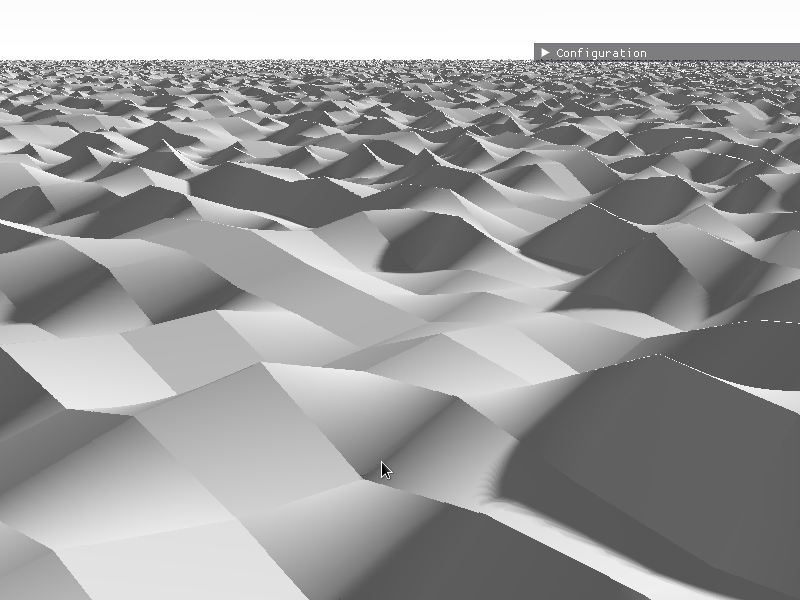
\includegraphics[width=0.65\textwidth]{./graf/ilin-edges.png}
\caption{Konfiguracja systemu budowy dla środowiska Visual Studio 16.}
\label{fig:linterp-edges}
\end{figure}


Rozwiązaniem tego problemu jest zastosowanie funkcji \ang{smoothstep} pozwalającej na uzyskanie wygładzonej interpolacji. W tym celu zmodyfikowano wzór \ref{eq:interp-biliniowa}, zastępując parametry $x$ i $y$ wykorzystując funkcję \ang{smoothstep} $n$-tego stopnia przedstawionej jako $S_n(p)$. Ostateczną postać funkcji przedstawia wzór \ref{eq:smooth-interp}. Obliczając gradient tej funkcji, można zauważyć, że wartości pochodnej dla każdego z czterech granicznych punktów jest równa $0$, dzięki czemu przejścia między grupami punktów nie są widoczne.

\begin{equation}
\label{eq:smooth-interp}
  \begin{split}
    f(x, y) & = a \\
       & + (b - a) S_n(x) \\
       & + (c - a) S_n(y) \\
       & + (a - b - c + d) S_n(x) S_n(y)
    \end{split}
\end{equation}

W programie wykorzystana została funkcja \ang{smoothstep} pierwszego stopnia, której postać jest widoczna na wzorze \ref{eq:smooth-interp-1}.

\begin{equation}
\label{eq:smooth-interp-1}
  \begin{split}
    S_1(x) = 3x^2 - 2x^3
  \end{split}
\end{equation}

Wynik zastosowania tego wzoru ukazuje rysunek \ref{fig:smooth-interp}.


\begin{figure}[H]
\centering
\subfloat[interpolacja biliniowa]{
  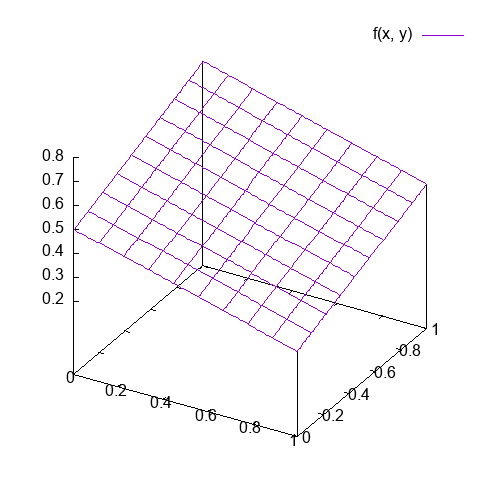
\includegraphics[width=0.5\textwidth]{./graf/plot/bilinear.png}
  \label{fig:lerp}
}
\subfloat[interpolacja wykorzystująca funkcję \ang{smoothstep} pierwszego stopnia]{
  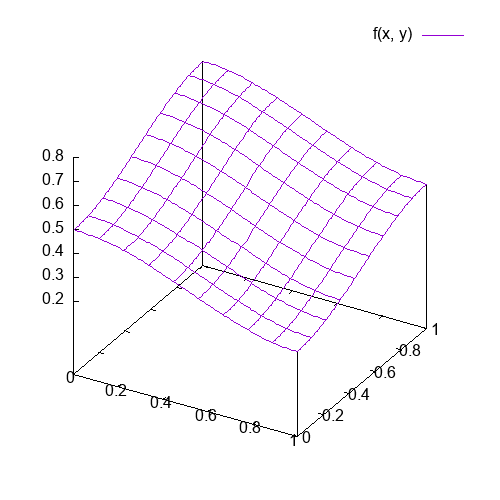
\includegraphics[width=0.5\textwidth]{./graf/plot/smooth.png}
  \label{fig:smooth-interp}
}
%% 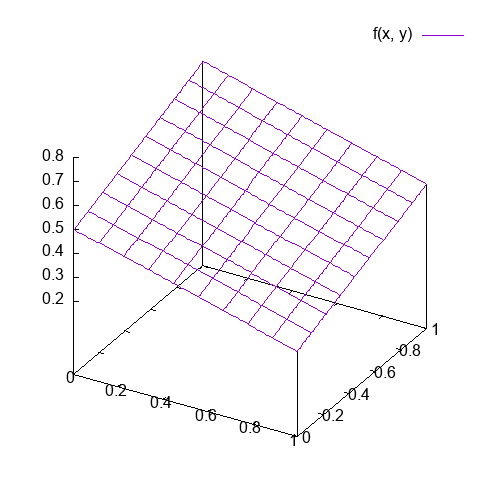
\includegraphics[width=0.65\textwidth]{./graf/plot/bilinear.png}
\caption{Porównanie wyników obu metod interpolacji między czterema punktami}
\label{fig:interpolacja}
\end{figure}

Uzyskany wynik jest zadowalający, jednak nadal nie przypomina naturalnego terenu. W celu poprawy jakości terenu można zastosować technikę o nazwie \ang{ułamkowe ruchy Browna} (\ang{fractional Brownian motion}, fBm)\cite{bib:bookofshaders}\cite{bib:Musgrave2003ProceduralFT}. Pożądany efekt można osiągnąć wykorzystując wzór \ref{eq:fbm}\cite{bib:iqfbm}, w którym $H$ jest wykładnikiem Hursta, a $N$ jest pożądaną ilością oktaw tej operacji.
\begin{equation}
\label{eq:fbm}
  \begin{split}
    fbm(p) = \sum^N_{k = 0} 2^{-Hk}f(2^kp)
  \end{split}
\end{equation}

W programie zastosowano wartość $H = 1$, gdyż wartość ta dała najbardziej realistyczne wyniki.
Zastosowanie stałej wartości $H$ daje bardziej uproszczony wzór, przedstawiony w postaci pseudokodu na rysunku \ref{fig:pseudokod:fbm}:

\begin{figure}[H]
\centering
\begin{lstlisting}[language=C]
float fbm(vec2 p) {
  float sum = 0.0;

  for (int i = 0; i < LAYERS; i++) {
    sum += pow(2, -i) * noise(pow(2, i) * p);
  }

  return sum;
}
\end{lstlisting}
\caption{Pseudokod funkcji \ang{fBm}.}
\label{fig:pseudokod:fbm}
\end{figure}

Kod z rysunku \ref{fig:pseudokod:fbm} został zmodyfikowany tak by zoptymalizować czas wykonania i uniknąć wykorzystania funkcji \ang{pow}\cite{bib:glslpow}. Wynikiem jest pseudokod z rysunku \ref{fig:pseudokod:fbm-opt}.

\begin{figure}[H]
\centering
%% \lstset{basicstyle=\ttfamily}
\begin{lstlisting}[language=C]
float fbm(vec2 p) {
  float sum = 0.0;
  float a = 1.0;

  for (int i = 0; i < LAYERS; i++) {
    sum += a * noise(p);
    p *= 2.0;
    a *= 0.5;
  }

  return sum;
}
\end{lstlisting}
\caption{Pseudokod funkcji \ang{fBm} po optymalizacji.}
\label{fig:pseudokod:fbm-opt}
\end{figure}

Po zastosowaniu powyższych działań uzyskano znacznie bardziej naturalny wynik. Dalsza analiza wygenerowanego terenu wykorzystując interpolację biliniową, przedstawiona na rysunku \ref{fig:fbm-bilin-align}, nasuwa wnioski, że wszystkie odkształcenia terenu biegną w jednej linii, co wpływa na naturalizm terenu. Aby uniknąć takiej sytuacji zmodyfikowano algorytm \ang{fBm} by oprócz skalowania współrzędnych punktu, zostały one także obrócone względem środka układu współrzędnych.

\begin{figure}
\centering
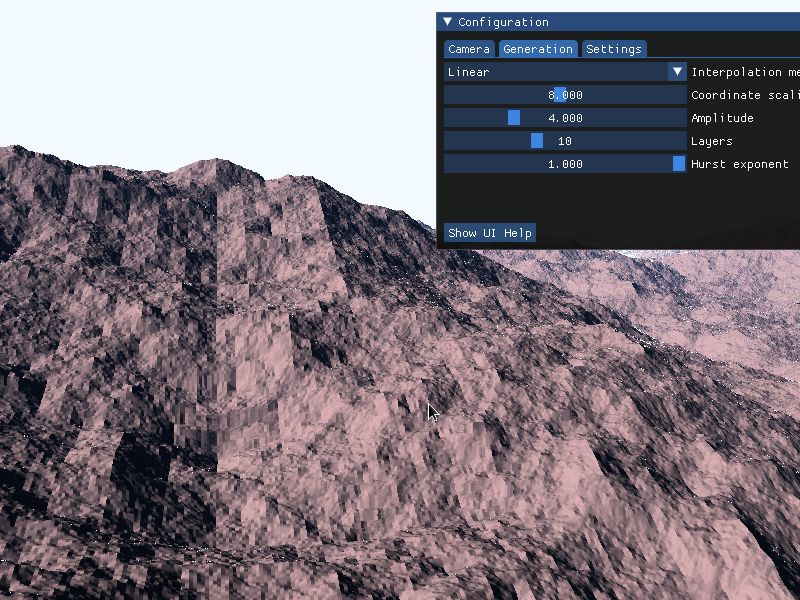
\includegraphics[width=1\textwidth]{./graf/fbm-bilin.png}
\caption{Wynik zastosowania \ang{fBm} dla 10 oktaw, z wykorzystaniem interpolacji biliniowej.}
\label{fig:fbm-bilin-align}
\end{figure}

%% \begin{itemize}
%% \item sformułowanie problemu
%% \item osadzenie tematu w kontekście aktualnego stanu wiedzy (\ang{state of the art}) o poruszanym problemie
%% \item  studia literaturowe \cite{bib:artykul,bib:ksiazka,bib:konferencja,bib:internet} -  opis znanych rozwiązań (także opisanych naukowo, jeżeli problem jest poruszany w publikacjach naukowych), algorytmów,
%% \end{itemize}


%% Wzory
%% \begin{align}
%% y = \frac{\partial x}{\partial t}
%% \end{align}
%% jak i pojedyncze symbole $x$ i $y$  składa się w trybie matematycznym.
 % analiza tematu 

% TODO
\chapter{Wymagania i narzędzia}
\label{ch:wymagania-i-narzedzia}

\begin{itemize}
\item wymagania funkcjonalne i niefunkcjonalne
\item przypadki użycia (diagramy UML) -- dla prac, w których mają zastosowanie
\item opis narzędzi, metod eksperymentalnych, metod modelowania itp.
\item metodyka pracy nad projektowaniem i implementacją -- dla prac, w których ma to zastosowanie
\end{itemize}
 % Wymagania i narzędzia

% TODO
\chapter{Specyfikacja zewnętrzna}
\label{ch:04}

\section{Wymagania sprzętowe i programowe}

Program wykorzystuje potok programowalny biblioteki OpenGL oraz jednostki cieniujące napisane w~języku GLSL w wersji 3.30. Oznacza to, że~system użytkownika musi posiadać kartę graficzną wspierającą OpenGL co najmniej w~wersji 3.3.
Dodatkowo program wykorzystuje następujące biblioteki, których kod źródłowy znajduje się wewnątrz projektu:
\begin{itemize}
\item GLAD
\item GLFW
\item GLM
\item Dear ImGui
\end{itemize}

Projekt został skompilowany i~przetestowany przy wykorzystaniu kompilatora g++
w~wersji 12.2.0 na~systemie Linux. Kompilacja programu odbywa się przy pomocy narzędzia CMake.

\section{Sposób instalacji}
\subsection{System Linux}
Przykład kompilacji programu został wykonany przy wykorzystaniu systemu Ubuntu 22.04. Pierwszym krokiem jest instalacja narzędzi takich jak program CMake, kompilator języka C i C++, itp. oraz instalacja wymaganych bibliotek.
Do tego celu wykorzystane są następujące polecenia
\begin{figure}[H]
\lstset{basicstyle=\ttfamily, language=bash}
\begin{lstlisting}[language=bash]
  sudo apt install cmake
  sudo apt install build-essential
  sudo apt install xorg-dev
  sudo apt install git
\end{lstlisting}
\end{figure}

Następnym krokiem jest pobranie repozytorium git projektu. Istotnym jest, by pobrać repozytorium rekurencyjnie, gdyż dołączone biblioteki zostały dodane do repozytorium jako submoduły. Można tego dokonać poleceniem
\begin{lstlisting}[language=bash]
  git clone https://github.com/Rei-sen/raymarch-terrain --recursive
\end{lstlisting}
Alternatywnie, jeżeli repozytorium nie zostało pobrane rekurencyjnie, można zastosować polecenia
\begin{lstlisting}[language=bash]
  git submodule init
\end{lstlisting}
a następnie
\begin{lstlisting}[language=bash]
  git submodule update
\end{lstlisting}
Ostatnim krokiem jest wygenerowanie plików reguł Makefile, a następnie
kompilacja projektu. Generacji plików reguł Makefile można dokonać wywołując następujące polecenie w głównym katalogu projektu
\begin{lstlisting}[language=bash]
  cmake -B build -S .
\end{lstlisting}
W celu kompilacji należy wykorzystać poniższe polecenie
\begin{lstlisting}[language=bash]
  cmake --build build
\end{lstlisting}
Końcowy plik wykonywalny o nazwie raymarch-terrain znajduje się w katalogu build.
\subsection{System Windows}
Pierwszym krokiem instalacji programu na systemie Windows jest pobranie
projektu z repozytorium github, które można znaleźć pod adresem
\url{https://github.com/Rei-sen/raymarch-terrain}. Podobnie jak przy instalacji programu na systemie Linux, repozytorium należy pobrać rekurencyjnie, z wszystkimi submodułami.
Dalszą część instalacji można dokonać w~środowisku Visual Studio lub
wykorzystując narzędzie CMake. Oba sposoby zostaną przedstawione poniżej.
\subsubsection{Instalacja przy wykorzystaniu środowiska Visual Studio}
Przed przystąpieniem do otwarcia projektu należy się upewnić, że
wsparcie systemu budowy CMake jest zainstalowane w środowisku Visual Studio.
Można tego dokonać w~instalatorze Visual Studio, jak na rysunku \ref{fig:vs-cmake-install}.

\begin{figure}
\centering
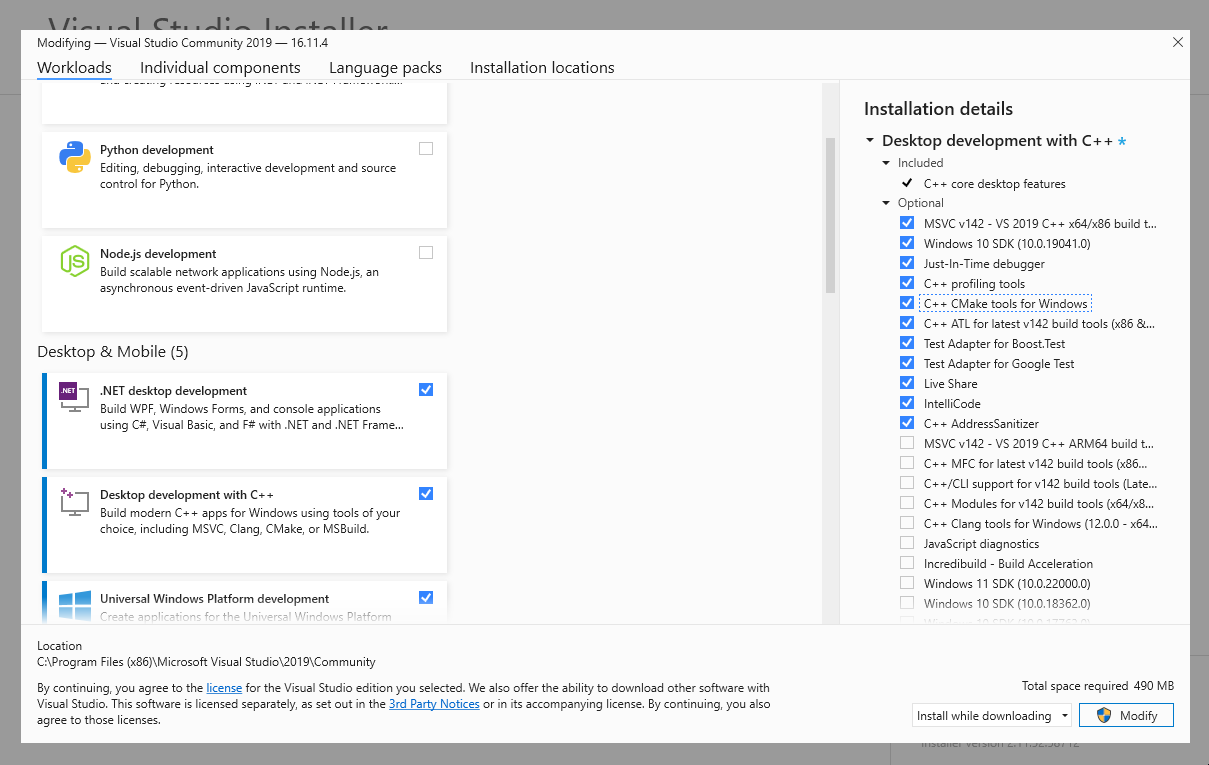
\includegraphics[width=1\textwidth]{./graf/vscmakeinstall.png}
\caption{Instalacja wsparcia systemu CMake w instalatorze środowiska Visual Studio.}
\label{fig:vs-cmake-install}
\end{figure}

Po zweryfikowaniu instalacji wsparcia systemu CMake należy uruchomić środowisko Visual Studio, a następnie wybrać opcję \ang{Open local folder}. Kolejnym krokiem jest wybranie głównego folderu projektu. Po otwarciu projektu i~ukończeniu generacji środowiska CMake, należy zmienić opcję \ang{Select startup item} na raymarcher.exe. Po wykonaniu powyższych kroków, projekt można budować oraz kompilować jak zwykły projekt środowiska Visual Studio.

\subsubsection{Instalacja z wykorzystaniem narzędzia CMake}
Pierwszym etapem jest instalacja narzędzia CMake, które można znaleźć pod adresem \url{https://cmake.org}.
Następnie należy uruchomić narzędzie CMake w trybie graficznym.
Kolejnym etapem jest wybór głównego katalogu projektu oraz katalogu budowy, w którym znajdą się końcowe pliki binarne.
Jako główny katalog projektu należy wskazać katalog, w którym znajduje się plik CMakeLists.txt.
Jako folder budowy został utworzony nowy folder o nazwie \ang{build} w głównym folderze projektu.
Przykład powyższych kroków został przedstawiony na rysunku \ref{fig:cmake-win}.
\begin{figure}[H]
\centering
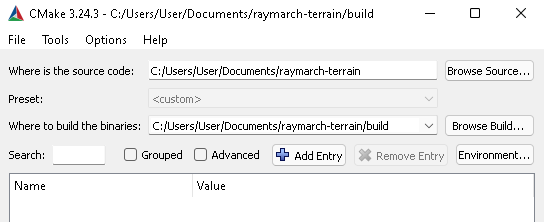
\includegraphics[width=1\textwidth]{./graf/cmake-win.png}
\caption{Wybór folderu projektu oraz folderu budowy narzędziu graficznym CMake.}
\label{fig:cmake-win}
\end{figure}
Kolejnym etapem jest konfiguracja systemu budowy, której można dokonać przyciskiem \ang{Configure}, a następnie wybierając (odpowiednie, interesujące nas) docelowe środowisko programistyczne. Rysunek \ref{fig:cmake-conf} przedstawia przykładową konfigurację dla środowiska Visual Studio 16 dla systemów 64-bitowych.

\begin{figure}[H]
\centering
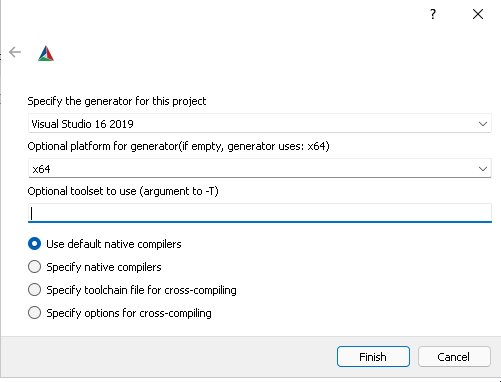
\includegraphics[width=1\textwidth]{./graf/cmake-conf.png}
\caption{Konfiguracja środowiska programistycznego.}
\label{fig:cmake-conf}
\end{figure}

Następnie należy wygenerować pliki budowy, wykorzystując przycisk \ang{Generate}.
Ostatnim etapem jest otwarcie projektu poprzez pliki znajdujące się w folderze budowy lub poprzez przycisk \ang{Open Project} w oknie programu CMake. W dalszej kolejności należy dokonać kompilacji programu, korzystając z wcześniej wybranego środowiska programistycznego.

\section{Sposób obsługi}
Po uruchomieniu program przedstawia prosty interfejs użytkownika, widoczny na~rysunku \ref{fig:ui}. Cały
obszar okna wykorzystywany jest do wyświetlania renderowanego terenu.
Dodatkowo wewnątrz okna renderowany jest obszar zawierający pola
pozwalające na zmianę parametrów związanych z renderowaniem oraz generacją
terenu. Użytkownik ma możliwość poruszania kamerą korzystając z klawiszy W, S, A oraz D. Zmiana orientacji kamery jest możliwa poprzez poruszanie myszką, gdy wciśnięty jest lewy przycisk myszki. Szczegółowe informacje dotyczące korzystania z interfejsu użytkownika można uzyskać naciskając przycisk \ang{Show UI Help}. Program można zakończyć poprzez naciśnięcie przycisku Escape lub zamknięcie okna.

\begin{figure}[H]
\centering
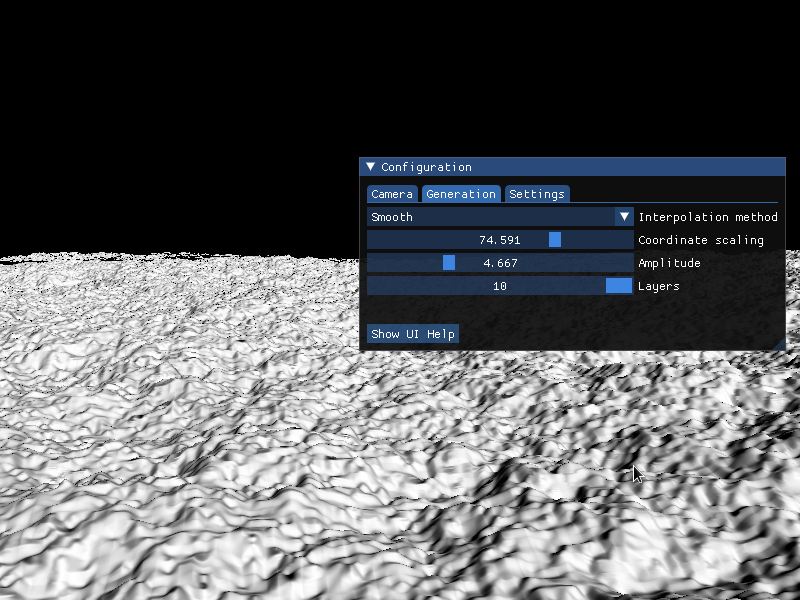
\includegraphics[width=0.95\textwidth]{./graf/ui.png}
\caption{Interfejs użytkownika}
\label{fig:ui}
\end{figure}

\section{Przykład działania}
Program daje użytkownikowi szeroki zakres ustawień związanych z renderowaniem oraz generowaniem terenu. Jedną z takich możliwości jest kontrola ustawień kamery w~zakładce \ang{Camera}, lista dostępnych ustawień:

\begin{itemize}
\item Position - współrzędne, w których znajduje się kamera,
\item FOV - pole widzenia kamery podane w stopniach,
\item Orientation - orientacja kamery:
  \begin{itemize}
    \item Horizontal - obrócenie kamery względem osi Y,podane w radianach,
    \item Vertical - obrócenie kamery względem osi X, podane w radianach.
  \end{itemize}
\end{itemize}

Wygenerowanie pożądanego ukształtowania terenu umożliwione jest przez następujące opcje:

\begin{itemize}
\item Terrain - Ustawienia związane z ukształtowaniem terenu:
  \begin{itemize}
    \item Max terrain rendering steps - maksymalna ilość kroków, renderowania terenu
    \item Interpolation method - Metoda interpolacji wysokości terenu:
      \begin{itemize}
        \item Linear - interpolacja biliniowa,
        \item Smooth - interpolacja z wykorzystaniem funkcji. \ang{smoothstep}
      \end{itemize}
    \item Coordinate scaling - skalowanie współrzędnych X oraz Z,
    \item Amplitude - skalowanie wysokości terenu,
    \item Layers - ilość warstw wykorzystane w technice \ang{fBm},
    \item Layer rotation - Obrócenie współrzędnych punktu dla każdej warstwy w~technice \ang{fBm}, podane w radianach,
    \item Hurst exponent - wykładnik Hurst'a, wykorzystany w technice \ang{fBm},
    \item Ground color - kolor terenu.
  \end{itemize}
\item Sky color - kolor nieba,
\item Sun direction - kierunek światła, podany w radianach,
\item Grass - parametry związane z trawą:
  \begin{itemize}
    \item Grass transition start - wartość współrzędnej Y wektora normalnego, od której rozpoczyna się trawa,
    \item Grass transition end - wartość współrzędnej Y wektora normalnego, od której trawa ma pełny kolor,
    \item Grass color - kolor trawy.
  \end{itemize}
\item Trees - opcje związane z generacją drzew:
  \begin{itemize}
    \item Max tree rendering steps - maksymalna ilość kroków renderowania drzew,
    \item Tree spacing - rozmiar odstępu między drzewami,
    \item Tree radius - szerokość drzew,
    \item Tree height - wysokość drzew,
    \item Tree height offset - przesunięcie drzew w pionie,
    \item Tree layers - ilość warstw odkształceń drzew,
    \item Tree distortion coordinate - skalowanie współrzędnych odkształceń drzew,
    \item Tree distortion amplitude - rozmiar odkształceń drzew,
    \item Tree color - zakres kolorów drzew,
    \item Tree surface flatness - kontrola jak płaski musi być teren by wyświetlić drzewa.
  \end{itemize}
\item Clouds - konfiguracja generacji chmur:
  \begin{itemize}
    \item Max cloud rendering steps - maksymalna ilość kroków renderowania chmur,
    \item Cloud altitude - wysokość na jakiej renderowane są chmury,
    \item Cloud height - wysokość chmur,
    \item Cloud coordinate scaling - skalowanie współrzędnych X oraz Z,
    \item Cloud amplitude - rozmiar odkształceń chmurRozwiązanie to d
    \item Cloud density scaling - gęstość chmur,
    \item Cloud layers - ilość warst wykorzystanych w technice \ang{fBm}.
  \end{itemize}
\end{itemize}

Konfiguracja związana z renderowaniem odbywa się poprzez następujące ustawienia:
\begin{itemize}
\item Enable shadows - wyświetlanie cieni,
\item Soft shadows - miękkie cienie,
\item Soft shadow range - rozmiar miękkich cieni,
\item Numerical normals - obliczenie wektorów normalnych przy wykorzystaniu metod numerycznych,
\item Enable sun glare - blask słońca,
\item Sun glare color - kolor blasku słońca,
\item Render raymarching iterations - wyświetlenie wizualizacji iteracji algorytmu raymarching,
\item Max raymarching iterations - maksymalna ilość iteracji wizualizacji.
\end{itemize}

Pozostałe opcje, inne niż związane z renderowaniem oraz generacją terenu, znajdują się w zakładce \ang{Settings}:

\begin{itemize}
\item Camera speed - szybkość poruszania kamerą,
\item Mouse sensitivity - czułość myszki.
\end{itemize}
%% \begin{itemize}
%% \item  wymagania sprzętowe i programowe
%% \item  sposób instalacji
%% \item  sposób aktywacji
%% \item  kategorie użytkowników
%% \item  sposób obsługi
%% \item  administracja systemem
%% \item  kwestie bezpieczeństwa
%% \item  przykład działania
%% \item  scenariusze korzystania z systemu (ilustrowane zrzutami z ekranu lub generowanymi dokumentami)
%% \end{itemize}

%%%%%%%%%%%%%%%%%%%%%
%% RYSUNEK Z PLIKU
%
%\begin{figure}
%\centering
%
\includegraphics[width=0.5\textwidth]{./graf/politechnika_sl_logo_bw_pion_pl.pdf}
%\caption{Podpis rysunku zawsze pod rysunkiem.}
%\label{fig:etykieta-rysunku}
%\end{figure}
%Rys. \ref{fig:etykieta-rysunku} przestawia …
%%%%%%%%%%%%%%%%%%%%%
%
%%%%%%%%%%%%%%%%%%%%%
%% WIELE RYSUNKÓW
%
%\begin{figure}
%\centering
%\begin{subfigure}{0.4\textwidth}
%    
\includegraphics[width=\textwidth]{./graf/politechnika_sl_logo_bw_pion_pl.pdf}
%    \caption{Lewy górny rysunek.}
%    \label{fig:lewy-gorny}
%\end{subfigure}
%\hfill
%\begin{subfigure}{0.4\textwidth}
%    
\includegraphics[width=\textwidth]{./graf/politechnika_sl_logo_bw_pion_pl.pdf}
%    \caption{Prawy górny rysunek.}
%    \label{fig:prawy-gorny}
%\end{subfigure}
%
%\begin{subfigure}{0.4\textwidth}
%    
\includegraphics[width=\textwidth]{./graf/politechnika_sl_logo_bw_pion_pl.pdf}
%    \caption{Lewy dolny rysunek.}
%    \label{fig:lewy-dolny}
%\end{subfigure}
%\hfill
%\begin{subfigure}{0.4\textwidth}
%    
\includegraphics[width=\textwidth]{./graf/politechnika_sl_logo_bw_pion_pl.pdf}
%    \caption{Prawy dolny rysunek.}
%    \label{fig:prawy-dolny}
%\end{subfigure}
%
%\caption{Wspólny podpis kilku rysunków.}
%\label{fig:wiele-rysunkow}
%\end{figure}
%Rys. \ref{fig:wiele-rysunkow} przestawia wiele ważnych informacji, np. rys. \ref{fig:prawy-gorny} jest na prawo u góry.
%%%%%%%%%%%%%%%%%%%%%


 
%% \begin{figure}
%% \centering
%% \begin{tikzpicture}
%% \begin{axis}[
%%     y tick label style={
%%         /pgf/number format/.cd,
%%             fixed,   % po zakomentowaniu os rzednych jest indeksowana wykladniczo
%%             fixed zerofill, % 1.0 zamiast 1
%%             precision=1,
%%         /tikz/.cd
%%     },
%%     x tick label style={
%%         /pgf/number format/.cd,
%%             fixed,
%%             fixed zerofill,
%%             precision=2,
%%         /tikz/.cd
%%     }
%% ]
%% \addplot [domain=0.0:0.1] {rnd};
%% \end{axis}
%% \end{tikzpicture}
%% \caption{Podpis rysunku po rysunkiem.}
%% \label{fig:2}
%% \end{figure}
 % [Właściwy dla kierunku -- np. Specyfikacja zewnętrzna]

% TODO
\chapter{Specyfikacja wewnętrzna}
\label{ch:05}

\section{Architektura systemu oraz przedstawienie idei}
Do realizacji projektu wykorzystano język C++ oraz bibliotekę OpenGL. Do kompilacji programu wykorzystano system budowy CMake. Kod odpowiadający za renderowanie obrazu napisany został w języku GLSL i wykonywany jest na karcie graficznej.
W pierwszej kolejności następuje utworzenie okna programu z wykorzystaniem biblioteki GLFW. Kolejny krok to inicjalizacja biblioteki OpenGL przy wykorzystaniu biblioteki GLAD i rozpoczęcie głównej pętli programu, w której obsługiwane są następujące czynności:
\begin{itemize}
\item obsługa klawiatury i myszki,
\item wyświetlenie i obsługa interfejsu użytkownika,
\item pobranie ustawień z interfejsu użytkownika i przekazanie ich do karty graficznej,
\item rozpoczęcie renderowania obrazu,
\item wyświetlenie uzyskanego obrazu.
\end{itemize}

Informacje o konfiguracji przekazywane są do jednostek cieniujących przy wykorzystaniu zmiennych typu \ang{uniform}. Jednostka cieniująca wierzchołków tworzy prostokąt pokrywający cały ekran, na którym odbywa się renderowanie obrazu. Całość renderowania odbywa się w jednostce cieniującej fragmentów. Pierwszym etapem jest obliczenie początkowej pozycji wiązki światła oraz jej kierunek dla każdego piksela. Uzyskane w ten sposób informacje o wiązce światła przekazywane są do fukncji \ang{render}. Funkcja ta odpowiada za następujące czynności:
\begin{itemize}
\item wywołanie funkcji algorytmu raymarching,
\item uzyskanie wektorów normalnych,
\item obliczenie koloru w zależności od rodzaju przeciętej wiązką światłą powierzchni,
\item obliczenia związane z cieniem i cieniowaniem,
\item obliczenie końcowego koloru danego piksela,
\item zastosowanie korekcji gamma.
\end{itemize}

\section{Przegląd ważniejszych klas oraz struktur danych}
W programie jedną najważniejszych jest klasa \ang{Application}, która odpowiada za inicjalizację całego programu oraz wykorzystanych bibliotek. Klasa ta zawiera główną pętlę programu, dodatkowo odpowiada za obsługę klawiatury i myszki. Deklaracja tej klasy została przedstawiona na rysunku \ref{fig:c++:application}.

\begin{figure}[H]
\centering
\begin{lstlisting}[language=C++]
class Application {
public:
  Application();
  ~Application();

  void run();
  void processInput();

private:
  Window win;
  UI ui;
  Config config;
  Renderer renderer;
};
\end{lstlisting}
\caption{Deklaracja klasy \ang{Application}.}
\label{fig:c++:application}
\end{figure}

Równie ważną jest klasa \ang{Renderer}, która odpowiada za inicjalizację podstawowych elementów niezbędnych do rozpoczęcia renderowania, kompilację jednostek cieniujących oraz ich połączenie. Ponadto umożliwia przekazywanie konfiguracji do jednostek cieniujących i rozpoczęcie renderowania. Rysunek \ref{fig:c++:renderer} przedstawia deklarację tej klasy.

\begin{figure}[H]
\centering
\begin{lstlisting}[language=C++]

class Renderer {
public:
  Renderer();
  ~Renderer();

  void update();
  void draw(const Config &c);

private:
  void updateUniforms(const Config &c);

  std::unique_ptr<GL::Program> program;
  std::unique_ptr<GL::Shader> vertexShader;
  GL::VAO vao;
};

\end{lstlisting}
\caption{Deklaracja klasy \ang{Renderer}.}
\label{fig:c++:renderer}
\end{figure}

Należy przytoczyć jeszcze klasę \ang{Window}, odpowiadającą za inicjalizację oraz obsługę okna aplikacji.
Deklaracja tej klasy widoczna jest na rysunku \ref{fig:c++:window}.

\begin{figure}[H]
\centering
\begin{lstlisting}[language=C++]
class Window {
public:
  Window();
  Window(unsigned width, unsigned height);
  ~Window();

  bool shouldClose() const;
  void pollEvents();
  void swapBuffers();

  operator GLFWwindow *() const { return w; }

private:
  GLFWwindow *w;
};
\end{lstlisting}
\caption{Deklaracja klasy \ang{Renderer}.}
\label{fig:c++:window}
\end{figure}

\section{Przegląd ważniejszych algorytmów}

Algorytm \ang{raymarching} jest najważniejszym z algorytmów wykorzystanych w programie. Jego rola polega na stopniowym
przesuwaniu wiązki światła do momentu przecięcia z dowolnym punktem powierzchni sceny. Sam algorytm wykorzystuje podane parametry, którymi są początkowa pozycja wiązki światła oraz jej kierunek. Jego końcowy wynik to odległość, którą musi przebyć wiązka by preciąć najbliższą powierzchnię. Algorytm ten wykorzystuje pomocniczą funkcję
\ang{map()}, która zwraca odległość między podanym punktem a najbliższą powierzchnią sceny. Kod tej funkcji zmienia się w zależności od renderowanej sceny, dlatego pominięto jej pseudokod.
Rysunek \ref{fig:pseudokod:raymarching} przedstawia pseudokod tego algorytmu.

\begin{figure}[H]
\centering
\begin{lstlisting}[language=C]
float raymarch(vec3 rayOrigin, vec3 rayDirection) {
  float distance = 0.0;

  for (int i = 0; i < MAX_STEPS; i++) {
    vec3 pos = rayOrigin + rayDirection * distance;
    float d = map(pos);
    distance += d;

    if (abs(d) < EPSILON) {
      return distance;
    }
    if (distance > MAX_DIST) {
      break;
    }
  }

  return MAX_DIST;
}
\end{lstlisting}
\caption{Pseudokod algorytmu renderowania metodą \ang{raymarching}.}
\label{fig:pseudokod:raymarching}
\end{figure}

Aby uzyskać efekt cienia, wykorzystano modyfikację tego algorytmu, w punkcie przecięcia wiązki wysyłana nowa wiązka skierowana w kierunku źródła światła. Na podstawie informacji o przecięciu ze sceną tej wiązki można określić czy dany punkt jest oświetlony. Dodatkowo wykorzystując wzór \ref{eq:r-shadow} można uzyskać efekt ,,miękkich'' cieni przy niewielkim koszcie obliczeń \cite{bib:iqsoftshadow}.
\begin{equation}
\label{eq:r-shadow}
r = min(\frac{map(p)}{\text{distance}})
\end{equation}
Rysunek \ref{fig:pseudokod:shadow} przedstawia pseudokod z wykorzystaniem ,,miękkich'' cieni.
\begin{figure}[H]
\centering
\begin{lstlisting}[language=C]

float shadow(vec3 rayOrigin) {

  float distance = 0.0;
  float minR = MAX_DIST;

  for (int i = 0; i < MAX_STEPS; i++) {
    vec3 pos = ro + sunDir * distance;
    float d = map(pos);

    float r = d/depth;
    minR = min(r, minR);

    depth += d;

    if (abs(d) < EPSILON)
      return 0.0;

    if (d > MAX_DIST) break;
  }
  return smoothstep(0.0, 1.0, minR);
}
\end{lstlisting}[H]
\caption{Pseudokod modyfikacji algorytmu \ang{raymarching} wykorzystany do obliczenia cieni.}
\label{fig:pseudokod:shadow}
\end{figure}

Różnice wynikające z zastosowania wzoru \ref{eq:r-shadow} przedstawia rysunek \ref{fig:shadow-comp}

\begin{figure}[H]
\centering
\subfloat[zwykłe cienie]{
  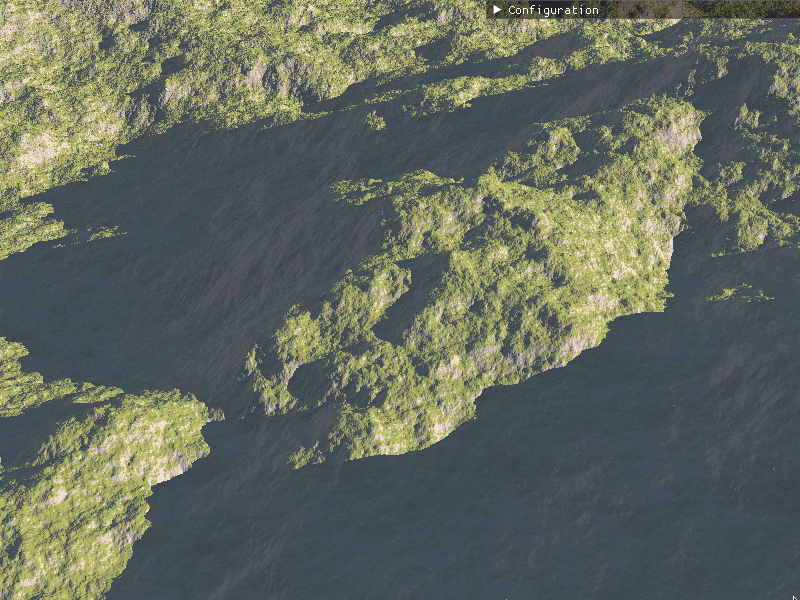
\includegraphics[width=0.5\textwidth]{./graf/shadow.png}
}
\subfloat[,,miękkie'' cienie]{
  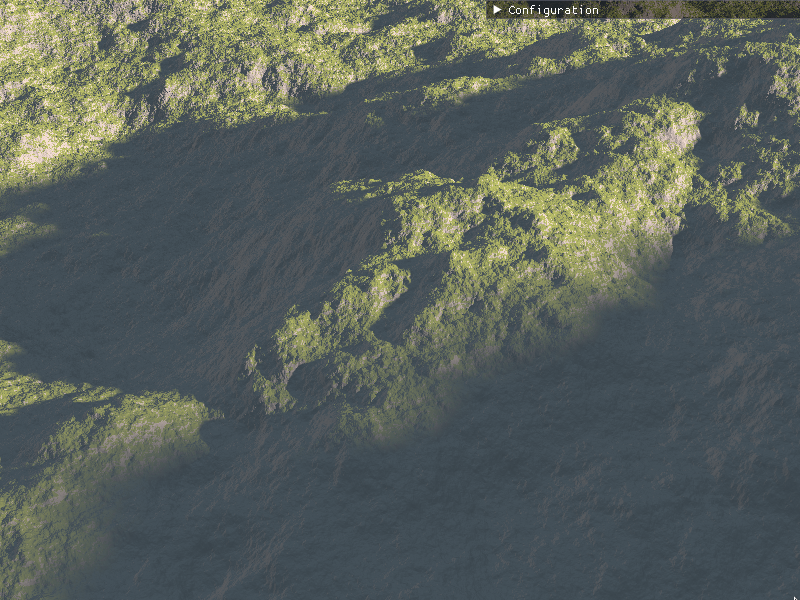
\includegraphics[width=0.5\textwidth]{./graf/shadowsmooth.png}
}
%% 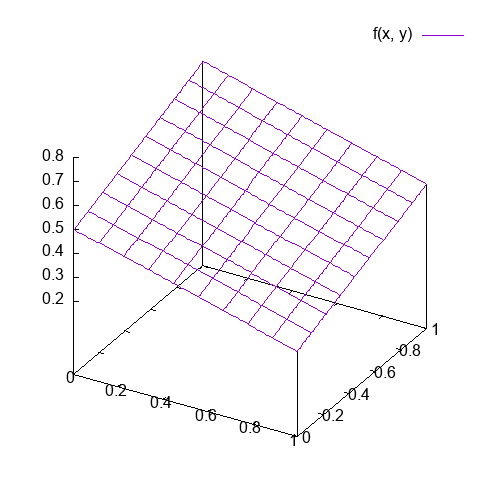
\includegraphics[width=0.65\textwidth]{./graf/plot/bilinear.png}
\caption{Porównanie wyników metod renderowania cieni}
\label{fig:shadow-comp}
\end{figure}


%% \subchapter{Szczególy implementacji wybranych fragmentów kodu}
%% \begin{i%% temize}
%% \item przedstawienie idei
%% \item architektura systemu
%% \item komponenty, moduły, biblioteki, przegląd ważniejszych klas (jeśli występują)
%% \item opis struktur danych (i organizacji baz danych)
%% \item przegląd ważniejszych algorytmów (jeśli występują)
%% \item szczegóły implementacji wybranych fragmentów, zastosowane wzorce projektowe
%% \item diagramy UML
%% \end{itemize}

% % % % % % % % % % % % % % % % % % % % % % % % % % % % % % % % % % %
% Pakiet minted wymaga odkomentowania w pliku config/settings.tex   %
% importu pakietu minted: \usepackage{minted}                       %
% i specjalnego kompilowania:                                       %
% pdflatex -shell-escape praca                                      %
% % % % % % % % % % % % % % % % % % % % % % % % % % % % % % % % % % %


%% Krótka wstawka kodu w linii tekstu jest możliwa, np.  \lstinline|int a;| (biblioteka \texttt{listings})% lub  \mintinline{C++}|int a;| (biblioteka \texttt{minted})
%% .
%% Dłuższe fragmenty lepiej jest umieszczać jako rysunek, np. kod na rys \ref{fig:pseudokod:listings}% i rys. \ref{fig:pseudokod:minted}
%% , a naprawdę długie fragmenty – w załączniku.


%% \begin{figure}
%% \centering
%% \begin{lstlisting}
%% class test : public basic
%% {
%%     public:
%%       test (int a);
%%       friend std::ostream operator<<(std::ostream & s,
%%                                      const test & t);
%%     protected:
%%       int _a;

%% };
%% \end{lstlisting}
%% \caption{Pseudokod w \texttt{listings}.}
%% \label{fig:pseudokod:listings}
%% \end{figure}

%% %\begin{figure}
%% %\centering
%% %\begin{minted}[linenos,frame=lines]{c++}
%% %class test : public basic
%% %{
%% %    public:
%% %      test (int a);
%% %      friend std::ostream operator<<(std::ostream & s,
%% %                                     const test & t);
%% %    protected:
%% %      int _a;
%% %
%% %};
%% %\end{minted}
%% %\caption{Pseudokod w \texttt{minted}.}
%% %\label{fig:pseudokod:minted}
%% %\end{figure}
 % [Właściwy dla kierunku -- np. Specyfikacja wewnętrzna]

% TODO
\chapter{Weryfikacja i walidacja}
\label{ch:06}

Z uwagi na implementację programu na karcie graficznej jako jednostkę cieniującą fragmentów, weryfikacja poprawności jego działania jest znacznie utrudniona. Programując w języku GLSL brak jest możliwości zastosowania testów jednostkowych, co spowodowało, że testowanie sprowadzało się do metody prób i błędów. Przeprowadzono porówynywania różnych technik i wzorów by uzyskać pożądany efekt. Ewentualne niepoprawne obliczenia są często niewidoczne mimo wydawało by się poprawnego działania. Jednym z takich problemów było obliczanie wektorów normalnych powierzchni, co spowodowane było niepoprawnym zastosowaniem wzoru. Błąd ten ujawnił się dopiero po implementacji cieni, gdy oświetlone powierzchnie były przyciemnione, sprawiały wrażenie, że były odwrócone od źródła światła. Defekt ten przedstawia rysunek \ref{fig:normals}.

\begin{figure}[H]
\centering
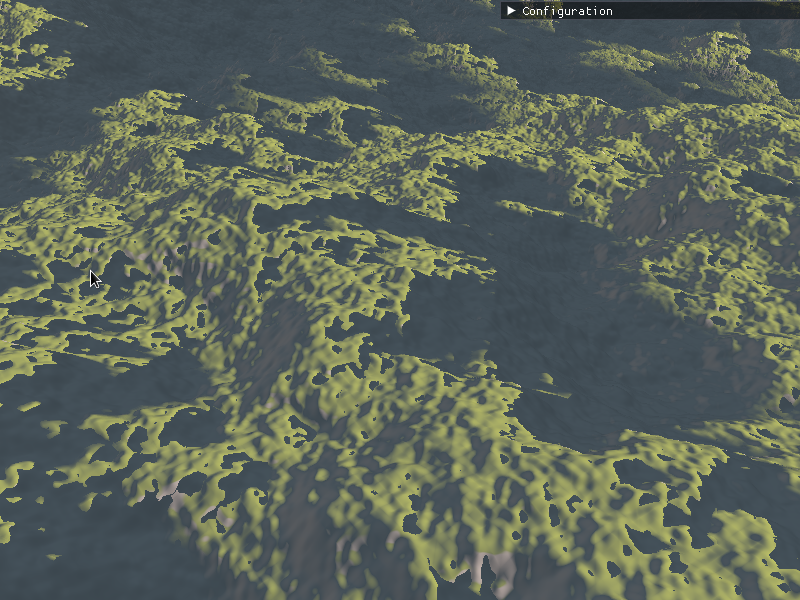
\includegraphics[width=1\textwidth]{./graf/norm.png}
\caption{Niepoprawne obliczanie wektorów normalnych.}
\label{fig:normals}
\end{figure}

%% \begin{itemize}
%% \item sposób testowania w ramach pracy (np. odniesienie do modelu V)
%% \item organizacja eksperymentów
%% \item przypadki testowe zakres testowania (pełny/niepełny)
%% \item wykryte i usunięte błędy
%% \item opcjonalnie wyniki badań eksperymentalnych
%% \end{itemize}

%% \begin{table}
%% \centering
%% \caption{Nagłówek tabeli jest nad tabelą.}
%% \label{id:tab:wyniki}
%% \begin{tabular}{rrrrrrrr}
%% \toprule
%% 	         &                                     \multicolumn{7}{c}{metoda}                                      \\
%% 	         \cmidrule{2-8}
%% 	         &         &         &        \multicolumn{3}{c}{alg. 3}        & \multicolumn{2}{c}{alg. 4, $\gamma = 2$} \\
%% 	         \cmidrule(r){4-6}\cmidrule(r){7-8}
%% 	$\zeta$ &     alg. 1 &   alg. 2 & $\alpha= 1.5$ & $\alpha= 2$ & $\alpha= 3$ &   $\beta = 0.1$  &   $\beta = -0.1$ \\
%% \midrule
%% 	       0 &  8.3250 & 1.45305 &       7.5791 &    14.8517 &    20.0028 & 1.16396 &                       1.1365 \\
%% 	       5 &  0.6111 & 2.27126 &       6.9952 &    13.8560 &    18.6064 & 1.18659 &                       1.1630 \\
%% 	      10 & 11.6126 & 2.69218 &       6.2520 &    12.5202 &    16.8278 & 1.23180 &                       1.2045 \\
%% 	      15 &  0.5665 & 2.95046 &       5.7753 &    11.4588 &    15.4837 & 1.25131 &                       1.2614 \\
%% 	      20 & 15.8728 & 3.07225 &       5.3071 &    10.3935 &    13.8738 & 1.25307 &                       1.2217 \\
%% 	      25 &  0.9791 & 3.19034 &       5.4575 &     9.9533 &    13.0721 & 1.27104 &                       1.2640 \\
%% 	      30 &  2.0228 & 3.27474 &       5.7461 &     9.7164 &    12.2637 & 1.33404 &                       1.3209 \\
%% 	      35 & 13.4210 & 3.36086 &       6.6735 &    10.0442 &    12.0270 & 1.35385 &                       1.3059 \\
%% 	      40 & 13.2226 & 3.36420 &       7.7248 &    10.4495 &    12.0379 & 1.34919 &                       1.2768 \\
%% 	      45 & 12.8445 & 3.47436 &       8.5539 &    10.8552 &    12.2773 & 1.42303 &                       1.4362 \\
%% 	      50 & 12.9245 & 3.58228 &       9.2702 &    11.2183 &    12.3990 & 1.40922 &                       1.3724 \\
%% \bottomrule
%% \end{tabular}
%% \end{table}
 % Weryfikacja i walidacja

% TODO
\chapter{Podsumowanie i wnioski}
W niniejszej pracy przedstawiono działanie metody \ang{raymarching}, wykorzystanej do~renderowania scen przedstawiających trójwymiarowy teren.
Technika ta pozwala na~tworzenie skomplikowanych scen, poprzez zastosowanie kombinacji wielu prostych funkcji matematycznych. Kształtowanie ternu odbywa się poprzez:
\begin{itemize}
\item Utworzenie siatki punktów z przypisanymi losowymi wartościami, odpowiadającymi wysokości terenu w danym miejscu,
\item Interpolację wartości między punktami,
\item Nałożenie na siebie wielu takich siatek, o zróżnicowanej częstotliwości oraz~amplitudzie ich punktów.
\end{itemize}

Przy tworzeniu programu zdecydowano się na zastosowanie technik dających gorsze efekty, jednak cechujących się lepszą wydajnością. Przykładem była implementacja drzew jako elementu sceny. Początkowo planowano indywidualną proceduralną generację poszczególnych drzew, jednak rozwiązanie to skutkowało znacznym spadkiem wydajności programu. W związku z powyższym zdecydowano się na rozwiązanie w postaci przedstawienia drzew jako elipsoid zniekształconych trójwymiarową funkcją \ang{fBm}.

Przedstawiony projekt można wzbogacić o dodatkowe elementy krajobrazu, na~przykład
poprzez generację struktur takich jak jeziora, rzeki, konstrukcje architektoniczne, itp. Program można rozbudować poprzez zastosowanie bardziej zaawansowanych technik obliczania koloru oraz światła, dla uzyskania obrazów bardziej odzwierciedlających rzeczywistość oraz zjawiska fizyczne. W niniejszej pracy nie zostały zastosowane techniki pozwalające ograniczyć efekty spowodowane \ang{aliasingiem}, jest~to~kolejna funkcjonalność, o którą można rozbudować ten projekt.

Przy tworzeniu programu napotkano wiele problemów, które między innymi związane były z podjęciem decyzji o renderowaniu na karcie graficznej. To z kolei znacząco utrudniło debugowanie programu. Przykładem takiej sytuacji był przez dłuższy czas niewykryty błąd matematyczny związany z obliczaniem wartości wektorów normalnych. Jego ujawnienie nastąpiło po implementacji cieni, co wymusiło dokonanie korekty zastosowanych wzorów.

Stworzony projekt miał na celu umożliwić syntezę obrazu jak najbardziej zbliżonego do naturalnego ukształtowania terenu. Zamiarem autora nie było uzyskanie fotorealizmu, a jedynie osiągnięcie przekonujących wyników. Przedstawione możliwości programu mogą być wykorzystane w grach i animacjach, a nawet po jego rozbudowie w filmach.
%% na karcie graficznej - debugowanie jest trudniejsz e


%% \begin{itemize}
%% \item uzyskane wyniki w świetle postawionych celów i zdefiniowanych wyżej wymagań
%% \item kierunki ewentualnych danych prac (rozbudowa funkcjonalna …)
%% \item problemy napotkane w trakcie pracy
%% \end{itemize}
 % Podsumowanie i wnioski

\backmatter 

%\bibliographystyle{plplain}  % bibtex
%\bibliography{biblio/biblio} % bibtex
\printbibliography           % biblatex 
\addcontentsline{toc}{chapter}{Bibliografia}

\begin{appendices}

% TODO
\chapter{Spis skrótów i symboli}

\begin{itemize}
\item[fBm] ułamkowe ruch Browna (ang. \ang{fractional Brownian motion})
\item[DNA] kwas deoksyrybonukleinowy (ang. \ang{deoxyribonucleic acid})
\item[MVC] model -- widok -- kontroler (ang. \ang{model--view--controller}) 
\item[$N$] liczebność zbioru danych
\item[$\mu$] stopnień przyleżności do zbioru
\item[$\mathbb{E}$] zbiór krawędzi grafu
\item[$\mathcal{L}$] transformata Laplace'a 
\end{itemize}
 % Spis skrótów i symboli

% TODO
\chapter{Źródła}

Jeżeli w pracy konieczne jest umieszczenie długich fragmentów kodu źródłowego, należy je przenieść w to miejsce.

\begin{lstlisting}
if (_nClusters < 1)
	throw std::string ("unknown number of clusters");
if (_nIterations < 1 and _epsilon < 0)
	throw std::string ("You should set a maximal number of iteration or minimal difference -- epsilon.");
if (_nIterations > 0 and _epsilon > 0)
	throw std::string ("Both number of iterations and minimal epsilon set -- you should set either number of iterations or minimal epsilon.");
\end{lstlisting}


% % % % % % % % % % % % % % % % % % % % % % % % % % % % % % % % % % % 
% Pakiet minted wymaga odkomentowania w pliku config/settings.tex   %
% importu pakietu minted: \usepackage{minted}                       %
% i specjalnego kompilowania:                                       %
% pdflatex -shell-escape praca                                      %
% % % % % % % % % % % % % % % % % % % % % % % % % % % % % % % % % % % 

%\begin{minted}[linenos,breaklines,frame=lines]{c++}
%if (_nClusters < 1)
%   throw std::string ("unknown number of clusters");
%if (_nIterations < 1 and _epsilon < 0)
%   throw std::string ("You should set a maximal number of iteration or minimal difference -- epsilon.");
%if (_nIterations > 0 and _epsilon > 0)
%   throw std::string ("Both number of iterations and minimal epsilon set -- you should set either number of iterations or minimal epsilon.");
%\end{minted}
 % Źródła

% TODO
\chapter{Lista dodatkowych plików, uzupełniających tekst pracy} 


W systemie do pracy dołączono dodatkowe pliki zawierające:
\begin{itemize}
\item źródła programu,
\item dane testowe,
\item film pokazujący działanie opracowanego oprogramowania lub zaprojektowanego i~wykonanego urządzenia,
\item itp.
\end{itemize}
 % Lista dodatkowych plików, uzupełniających tekst pracy

\listoffigures
\addcontentsline{toc}{chapter}{Spis rysunków}
\listoftables
\addcontentsline{toc}{chapter}{Spis tabel}
	
\end{appendices}

\end{document}


%% Finis coronat opus.

